%!TEX root=paper/paper.tex
\chapter{Basic C Language}\label{sec:basic_chapter}

\PM{Keywords}
由ANSI标准定义的C语言关键字共32个 :

\begin{table}
\begin{tabular}{|l|l|l|l|l|l|l|}
\hline
auto      & break  & case      & char    & const  	   & continue	  & default   \\
\hline
do        & double &  else     & enum    & extern      & float        & for       \\
\hline
goto      & if     & int       & long    & register    &  return      & short     \\
\hline
signed    & sizeof & static    & sturct  & switch      & typedef      & union     \\
\hline
unsigned  & void   & volatile  &  while  & \textit{inline}    & \textit{restrict}     & \textit{_Bool_Complex}   \\
\hline
\textit{_Imaginary} & \textit{_Alignas} & \textit{_Alignof}  & \textit{_Atomic}   & \textit{_Static_assert}  &  \textit{_Noreturn}  & \textit{_Thread_local}     \\
\hline
\textit{_Generic}  & & & & & &  \\
\hline
\end{tabular}
\end{table}

根据关键字的作用,可以将关键字分为\textit{数据类型关键字}和\textit{流程控制关键字}两大类。

\begin{enumerate}[label=\arabic*)]
	\item 基本数据类型(5个)
	\begin{enumerate}
		\item void: 声明函数无返回值或无参数,声明无类型指针,显式丢弃运算结果
		\item char: 字符型类型数据,属于整型数据的一种
		\item int: 整型数据,通常为编译器指定的机器字长
		\item float: 单精度浮点型数据
		\item double: 双精度浮点型数据
	\end{enumerate}
	\item 类型修饰关键字(4个)
	\begin{enumerate}
		\item short: 修饰int,短整型数据,可省略被修饰的int。
		\item long: 修饰int,长整形数据,可省略被修饰的int
		\item signed: 修饰整型数据,有符号数据类型
		\item unsigned: 修饰整型数据,无符号数据类型
	\end{enumerate}
	\item 复杂类型关键字(5个)
	\begin{enumerate}
		\item struct: 结构体声明
		\item union: 共用体声明
		\item enum: 枚举声明
		\item typedef: 声明类型别名
		\item sizeof: 得到特定类型或特定类型变量的字节大小
	\end{enumerate}
	\item 存储级别关键字(6个)
	\begin{enumerate}
		\item auto: 指定为自动变量,由编译器自动分配及释放。通常在栈上分配
		\item static: 指定为静态变量,分配在静态变量区,修饰函数时,指定函数作用域为文件内部
		\item register: 指定为寄存器变量,建议编译器将变量存储到寄存器中使用,也可以修饰函数形参,建议编译器通过寄存器而不是堆栈传递参数
		\item extern: 指定对应变量为外部变量,即在另外的目标文件中定义,可以认为是约定由另外文件声明的对象的一个``引用"
		\item const: 与volatile合称“cv特性”,指定变量不可被当前线程/进程改变(但有可能被系统或其他线程/进程改变)
		\item volatile: 与const合称“cv特性”,指定变量的值有可能会被系统或其他进程/线程改变,强制编译器每次从内存中取得该变量的值
	\end{enumerate}	
\end{enumerate}


   

%!TEX root=../paper/paper.tex
\section{Method}\label{sec:ccnn_method}

\PM{R-CNN}
We take the R-CNN \cite{Girshick-CVPR-2014} method as our point of departure.
As summarized in \autoref{fig:rcnn}, R-CNN starts with external region-of-interest proposals (ROIs), which are transformed to canonical size, and classified with a CNN, obtaining multi-class scores for each region.
After all batches of ROIs have been scored, they are post-processed with non-maximal suppression and other bounding box refinement to obtain the final detections.

\PM{Our method}
As summarized in \autoref{fig:combined}, we begin with the same ROI proposals, but first score all proposals with a quick-to-compute feature.
We then select a batch of highly-scoring ROIs and classify them with the CNN -- which is additionally sped up with cascaded structure.
After the batch is scored, we optionally re-score the remaining ROIs, and repeat the process until either time or regions are depleted.
The quick-to-compute feature is used to select batches of regions in a way that orders the regions most likely to contain ground truth objects earlier than other regions.
This process of region selection does not reject regions flat out, but reorders them to be processed later.

\PM{Region order}
We found that simply sorting the regions by score and taking batches in that sorted order results in poor performance, and can be worse than taking regions in an entirely random order, as the highest scoring regions may be highly overlapping with each other, and only result in one detection after non-maximal suppression and other post-processing of detections.
Instead, we put regions in random order, set a threshold for the quick-to-compute feature such that only half of the unprocessed regions score above it, take a batch of the above-threshold regions in their order, update the threshold, and repeat.

\begin{figure}[ht]
\begin{center}
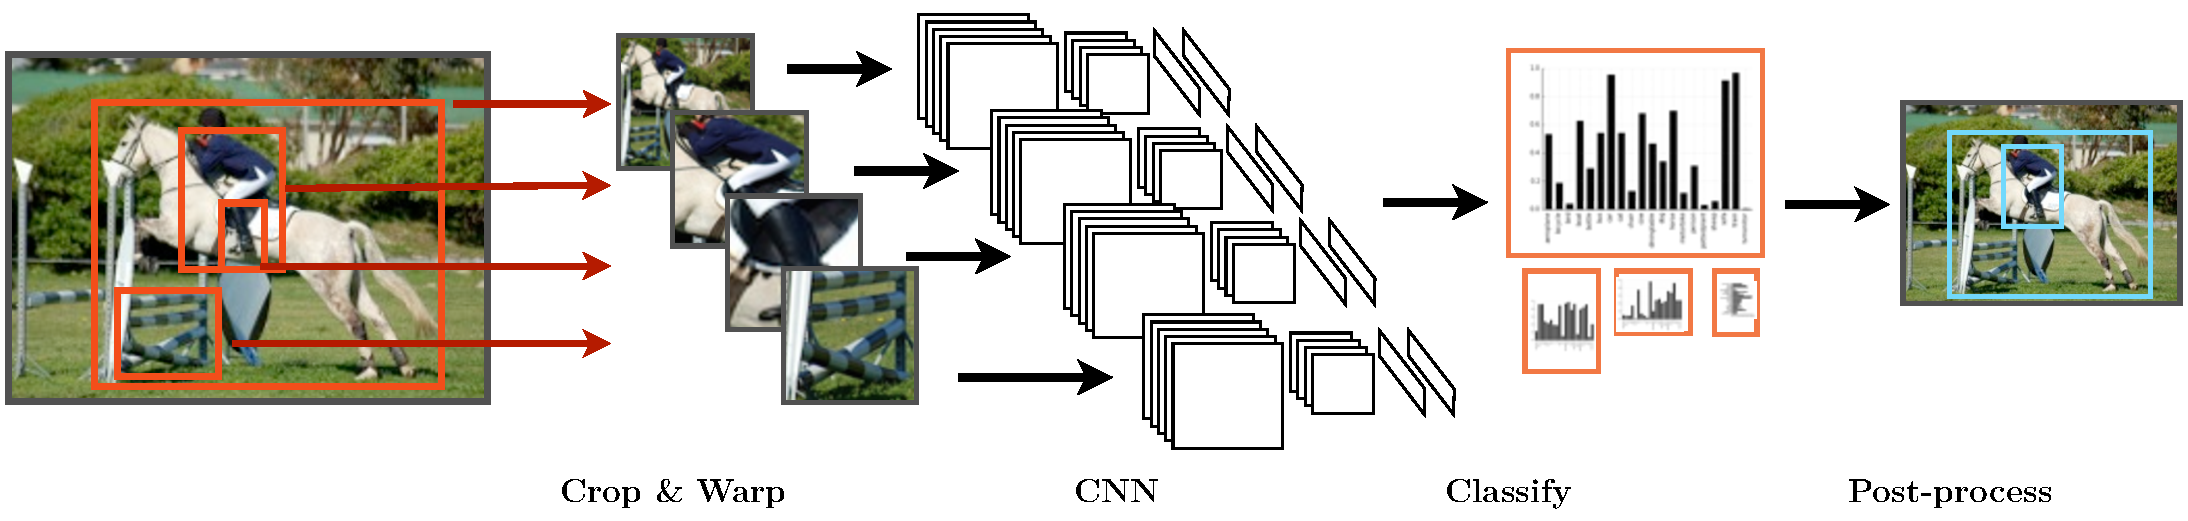
\includegraphics[width=0.98\columnwidth]{../ccnn/figures/rcnn.pdf}
\caption[
Summary of the R-CNN architecture.]{
R-CNN architecture: image regions are cropped, resized, and each one fed through a CNN.
The classifier outputs are post-processed to give the final detections.
}\label{fig:rcnn}
\end{center}
\end{figure}


\begin{figure}[ht]
\begin{center}
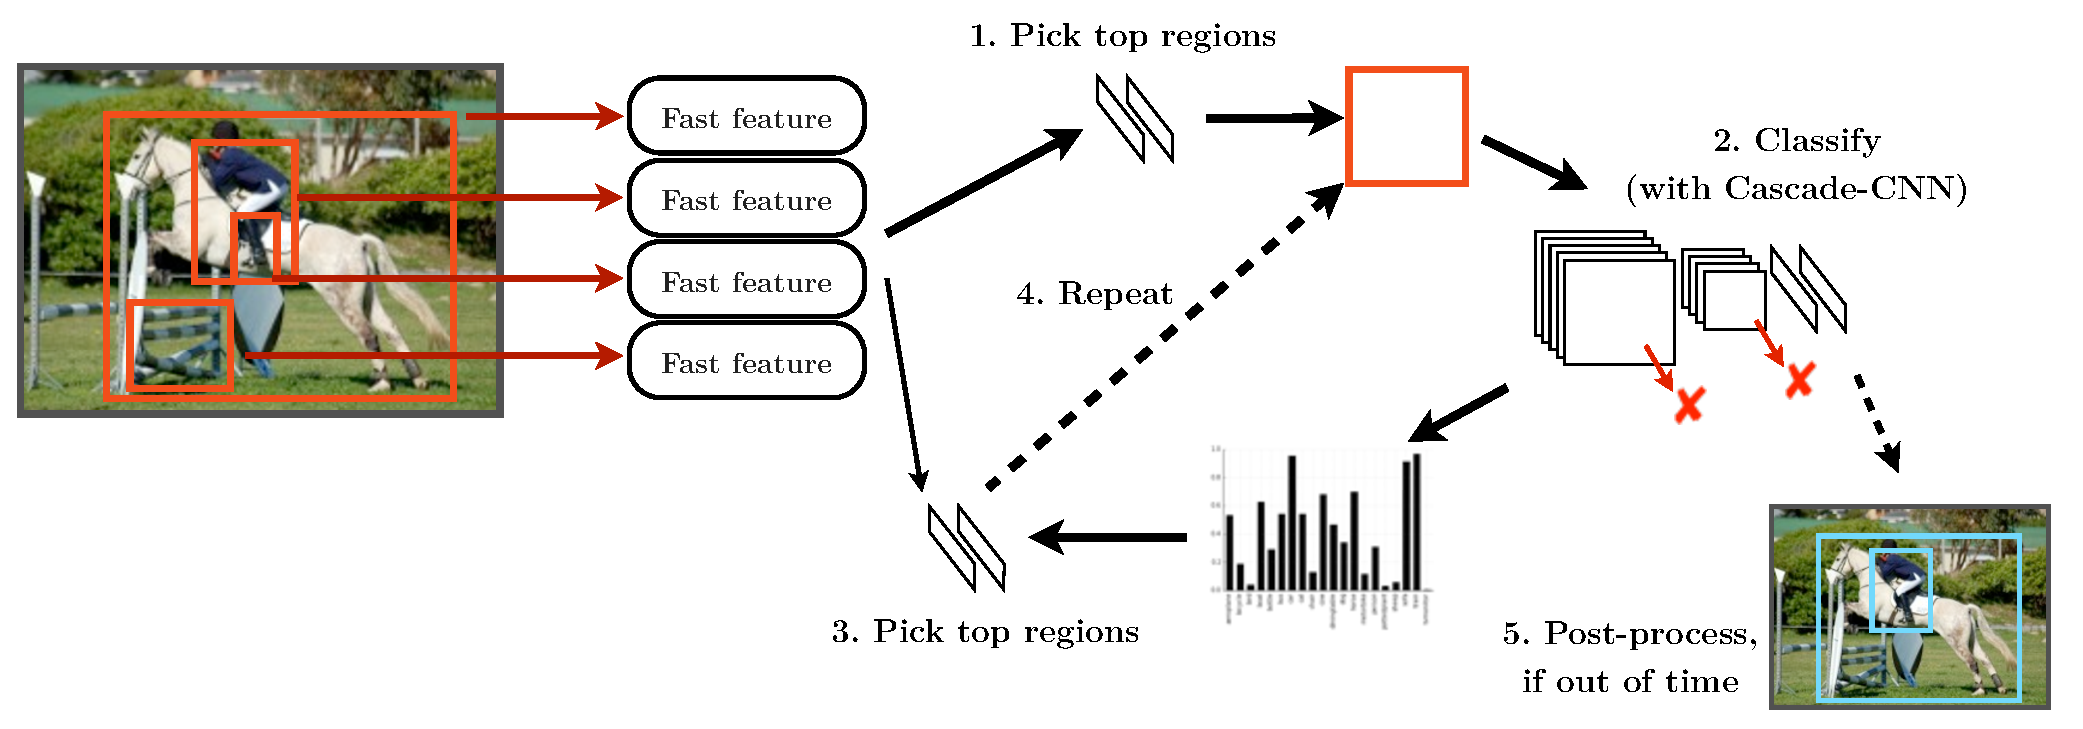
\includegraphics[width=0.98\columnwidth]{../ccnn/figures/combined.pdf}
\caption[
Summary of our method for dynamic region selection and cascaded CNN processing.]{
Our method scores each region of interest with a fast feature (we evaluate several), allowing us to pick promising regions first.
The regions are classified with the original CNN, or a sped-up Cascade-CNN.
The properties of the regions can play a role in selecting the next batch of regions.
}\label{fig:combined}
\end{center}
\end{figure}


\subsection{Quick-to-compute feature}

\PM{Region statistics}
For the first source of information, we consider statistics about ROI location and overlap with other regions.
For each ROI, we compute: its normalized location, its scale ($\sqrt{\text{width} \times \text{height}}$), aspect ratio ($\log \sqrt{\text{width} / \text{height}}$), and normalized counts of overlapping regions, at several PASCAL overlap thresholds (0, 0.2, 0.6).
This simple feature works suprisingly well for filtering regions to process first.

\PM{Pixel gradient}
In concatenation, we also consider the \emph{pixel gradient}, back-propagated throgh a classification CNN applied to the whole image.
This feature corresponds to a kind of saliency map, giving an estimate of the importance of each pixel to the final classification of the image.
Our method is independently developed, but agrees with the concurrently published work of \cite{Simonyan-ICLR-2014} quite closely.
Images are resized to square and classified with an ``AlexNet'' \cite{Krizhevsky-NIPS-2012} CNN fine-tuned on the PASCAL VOC classification dataset with multi-label loss.
(Unlike the ILSVRC, the PASCAL VOC is a multi-label prediction task, with at times multiple correct labels for an image.)
At test-time, the gradient at the top is with respect to the indicator function of the max-scoring class, and is back-propagated all the way to the pixels, where it is summed across channels.
A couple of example images are shown in \autoref{fig:gradient_examples}.
We compute an integral image on this pixel gradient map, allowing near-instant computation of sums in arbitrary regions.
For each region to be evaluated, we compute the image-normalized gradient sum, sums for each of four corners, and ratio of in-region vs. out-of-region sums.

\begin{figure}
\centering
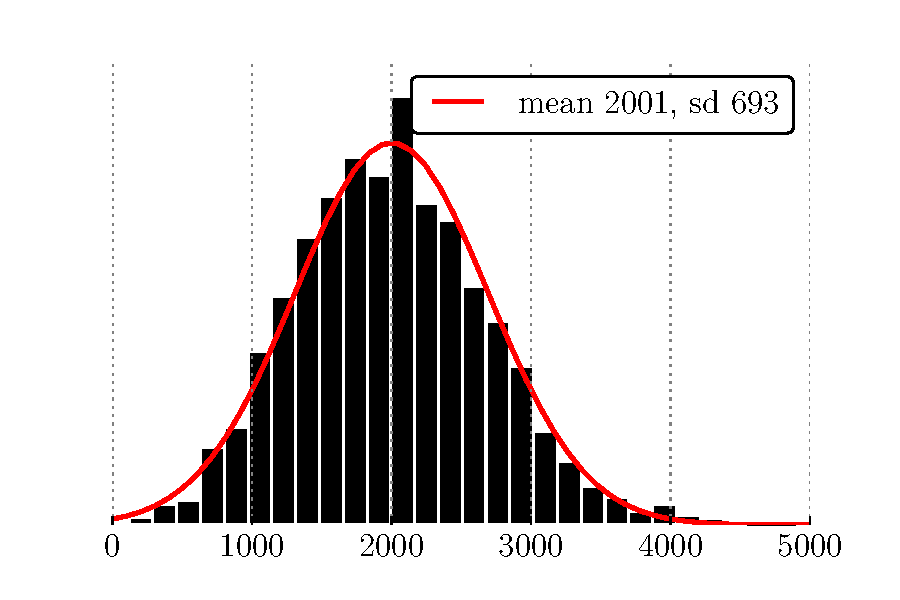
\includegraphics[width=.66\linewidth]{../ccnn/figures/roi_hist.pdf}
\caption{
Distribution of number of regions per image.
}\label{fig:roi_hist}
\end{figure}

\begin{figure}
\centering
\includegraphics[width=.66\linewidth]{../../figures/gradient_backprop.pdf}
\caption[Explanation of the gradient back-propagation quick feature.]{
As a quick feature, we back-propagate the gradient from the top classification layer all the way to the input pixels.
This induces a kind of saliency map on the image, which is useful signal for selecting image sub-regions to classify with the CNN.
}\label{fig:gradient_examples}
\end{figure}

\subsection{Cascade CNN}\label{sec:ccnn}

\PM{Motivation}
Despite the intentions of the region-proposal mechanism \parencite{Uijlings-IJCV-2013}, most ROIs that are scored in R-CNN do not contain any object of interest.
As in the classic cascade of \cite{Viola-IJCV-2004}, it would be useful to quickly reject these regions, without expending the full amount of computation on them.
The problem is that the deep neural network architecture is trained to always run all the way through.
We need to introduce a new primitive to enable early termination.

\PM{Method}
The Cascade CNN, shown in \autoref{fig:ccnn}, augments the CNN network with an ``Early Reject'' option: after some layers, the network decides whether to keep processing the input with the next layer.
Each reject layer is implemented as a fully-connected layer following a linear rectification, trained with dropout using logistic loss on foreground/background labels.
We first train an AlexNet-architecture network \parencite{Krizhevsky-NIPS-2012} on the ImageNet classification dataset.
This network is augmented with the Reject layers, its loss replaced with a multi-label cross-entropy loss, and fine-tuning on the PASCAL VOC training set is performed until loss stop decreasing (roughly 50000 iterations).
In training, all instances pass through all Reject layers.
After training, we set the reject thresholds to maintain at last 80\% recall at each stage, using a large sample of regions from images in the validation set containing positive and negative examples in equal proportion.

\PM{Implementation}
In the efficient implementation of CNNs we use (Caffe), there is a simple loop over each batch element in both CPU and GPU convolution code.
We modify this loop to simply not perform convolution on those elements that were rejected earlier in the cascade.
\footnote{While memory remains occupied in this scheme, we do not consider this a problem.}
Since most of the time is spent in the convolutional layers, we introduce a reject option after \texttt{pool1}, \texttt{pool2}, and \texttt{conv3}.
The last classification layer still outputs the full multi-class scores for the surviving regions.

\PM{Timing}
To estimate the saving on time by using the rejectors we timed the time spend to process 1000 regions (10 batches or 100) and the time expended in each of the first 3 layers:
\begin{itemize}
\item 1700 ms to process all the layers
\item 270 ms (15\%) in layer 1 (This includes \texttt{conv1}, \texttt{relu1}, \texttt{pool1}, \texttt{norm1})
\item 360 ms (20\%) in layer 2 (This includes \texttt{conv2}, \texttt{relu2}, \texttt{pool2}, \texttt{norm2})
\item 285 ms (15\%) in layer 3 (This includes \texttt{conv3}, \texttt{relu3})
\end{itemize}
Therefore the expected ``lifetimes'' of regions rejected after layer 1, layer 2, and layer 3 are  0.15, 0.35, and 0.5 of the total time taken per region.

\begin{figure}[h!]
\begin{center}
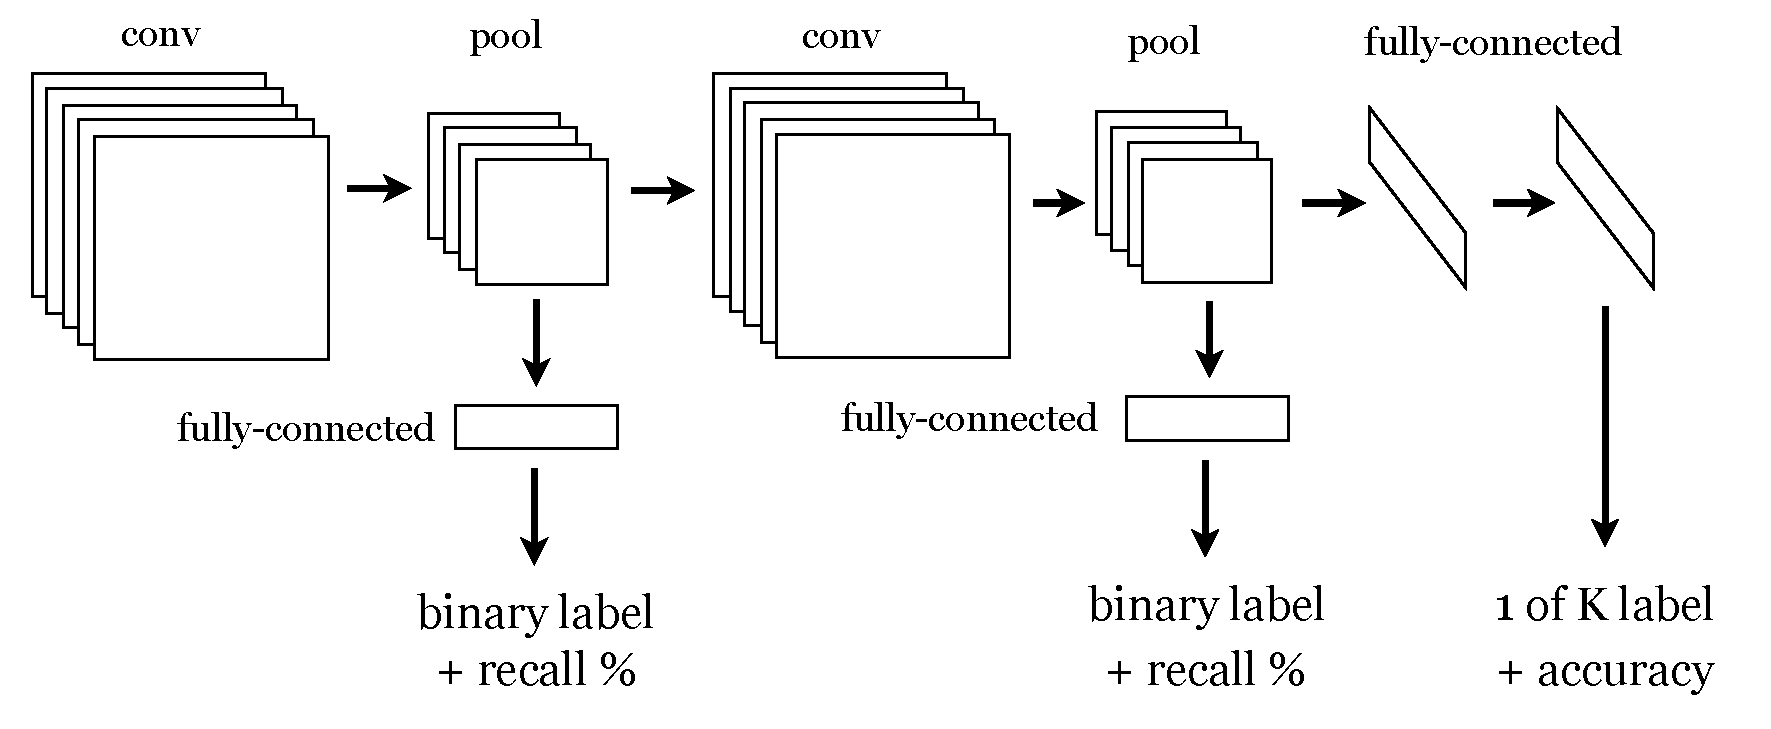
\includegraphics[width=0.98\columnwidth]{../ccnn/figures/ccnn-expanded.pdf}
\caption{
The Cascade CNN has a Reject option after computationally expensive layers, implemented as a binary prediction for reject/keep (background/foreground for our detection task).
The goal of the Reject layer is to maintain high recall while culling as much of the batch as possible, so that we can avoid doing as much convolution in the next layer.
}\label{fig:ccnn}
\end{center}
\end{figure}



%!TEX root=../paper/paper.tex
\section{Evaluation}\label{sec:ccnn_evaluation}

\PM{Dataset}
We evaluate on the standard object detection benchmark: the PASCAL VOC \cite{pascal-voc-2010}.
In all cases, the CNN region classifiers are trained on the PASCAL VOC 2007 trainval set.
The parameters of our methods are set by training or cross-validation on the VOC 2007 val set.
We evaluate on the VOC 2007 test set.
The result plots and details are shown in \autoref{fig:voc2007_results} and \autoref{tab:ccnn_results}.

\PM{Implementation}
The scoring function for the quick-to-compute features is trained by a logistic regression classifier onto the max PASCAL overlap with any ground truth window on the validation dataset.
The classifier is optimized by stochastic gradient descent, and its regularization parameter is cross-validated.
The R-CNN software was used as available in June 2014.
\footnote{\url{https://github.com/rbgirshick/rcnn}}
That software relies on Selective Search \cite{Uijlings-IJCV-2013} region proposals.
Different images are proposed different numbers of regions.
\autoref{fig:roi_hist} shows the distribution of number of regions on the validation set, with the parameters of the R-CNN.
An additional parameter is the size of each batch of regions that goes through the CNN.
We set batch size to 100 regions, and observe that it takes on average 500 ms to process them with the CNN.
In all experiments, we use Ubuntu 12.04, Intel i5 3.2GHz CPU, and NVIDIA Tesla K40 GPU.

%!TEX root=../paper/paper.tex
\begin{figure}[ht]
\begin{subfigure}[b]{\linewidth}
    \centering
    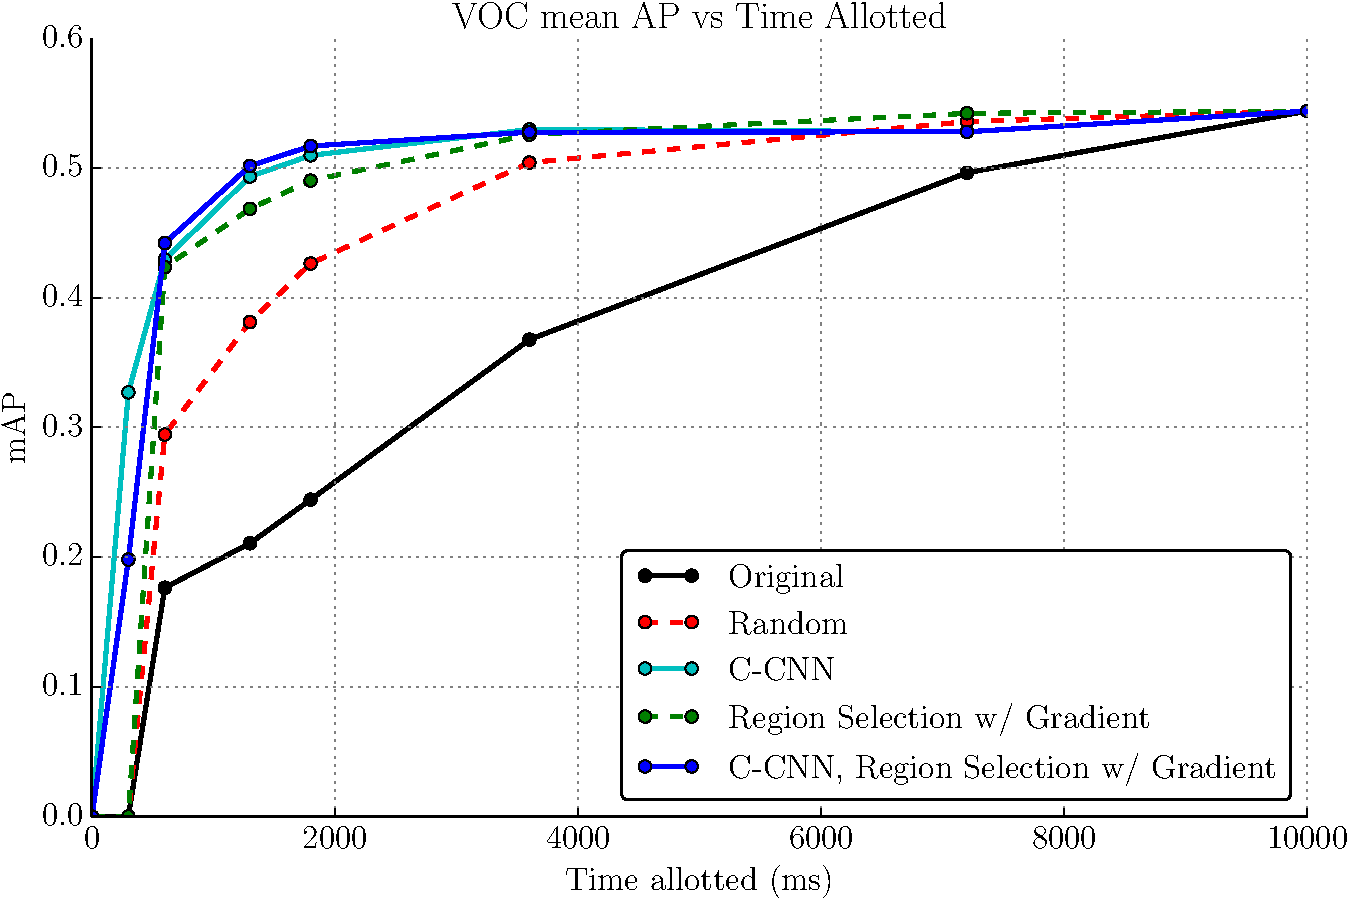
\includegraphics[width=.75\linewidth]{../ccnn/figures/_apvst_final.pdf}
    \caption{
Plotting Mean AP vs. Time Allotted allows comparison performance at a given time budget.
For example, at 1300 ms, random region selection gets about 0.42 mAP, while our best method (C-CNN with gradient-based region selection) obtains 0.50 mAP.
}\label{fig:apvst}
\end{subfigure}
\begin{subfigure}[b]{\linewidth}
    \centering
    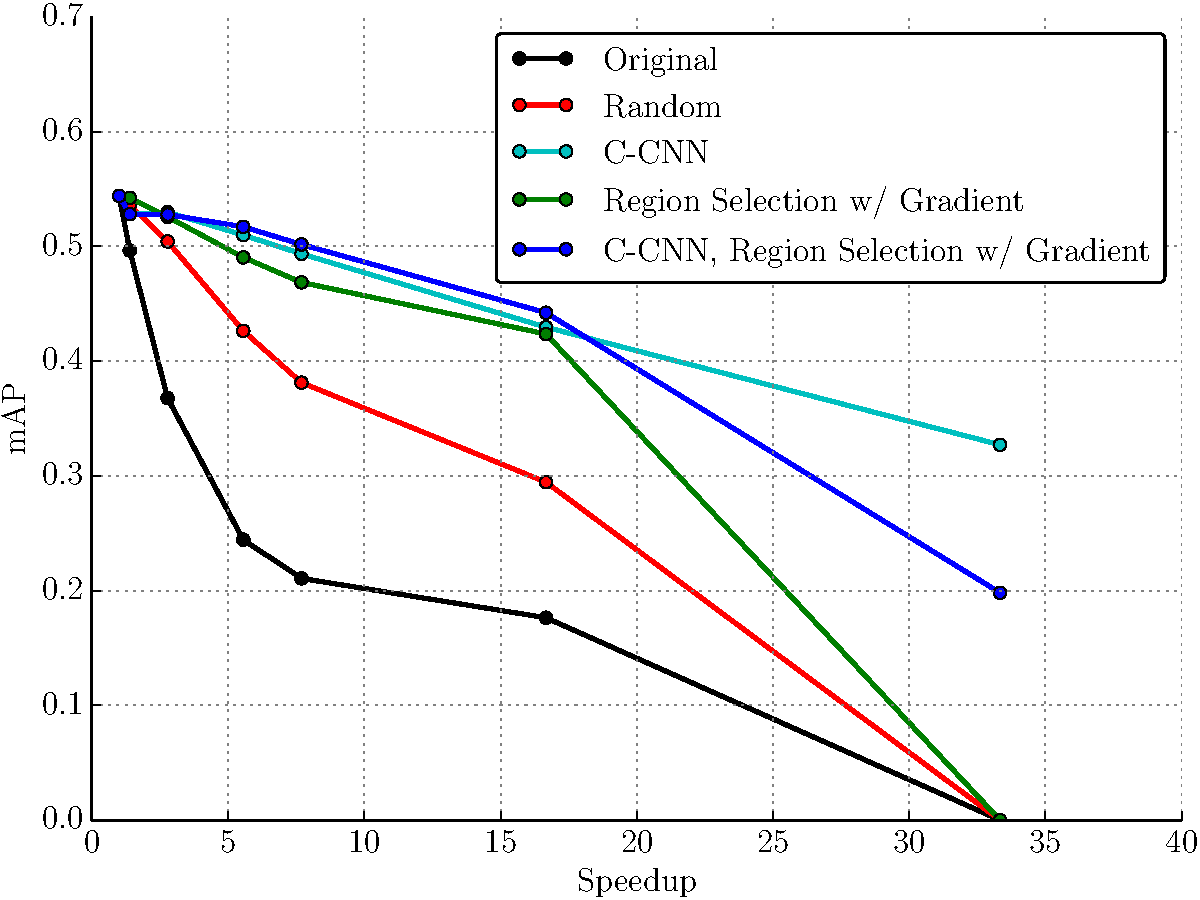
\includegraphics[width=.75\linewidth]{../ccnn/figures/_speedup_final_abs.pdf}
    \caption{
Plotting mean AP vs. speed-up factor allows comparison of speed-ups at a given mAP point.
For example, we can see that we should obtain mAP of 0.40 at around 20x speedup with our method.
}\label{fig:speedup}
\end{subfigure}
\caption{
Results of the Cascade CNN and other Anytime methods on the PASCAL VOC 2007 dataset.
}\label{fig:voc2007_results}
\end{figure}


\begin{table}[ht]
\centering
\caption{
Full table of AP vs. Time results on PASCAL VOC 2007.
Best performance for each time point is in bold.
}\label{tab:ccnn_results}
\small{
\begin{tabular}{lrrrrrrrr}
\toprule
Time allotted (ms)                  & 0 & 300            & 600            & 1300           & 1800           & 3600           & 7200           & 10000 \\
\midrule
Original                            & 0 & 0.000          & 0.176          & 0.211          & 0.244          & 0.368          & 0.496          & 0.544 \\
Random                              & 0 & 0.000          & 0.295          & 0.381          & 0.426          & 0.504          & 0.536          & 0.544 \\
C-CNN                               & 0 & \textbf{0.327} & 0.430          & 0.493          & 0.510          & 0.528          & 0.528          & - \\
Region Selection w/ Gradient        & 0 & 0.000          & 0.424          & 0.469          & 0.490          & 0.526          & \textbf{0.542} & 0.544 \\
C-CNN, Region Selection w/ Gradient & 0 & 0.198          & \textbf{0.442} & \textbf{0.502} & \textbf{0.517} & \textbf{0.528} & 0.528          & - \\
\bottomrule
\end{tabular}
}
\end{table}


The experimental settings are
\begin{description}
  \item[Original] \hfill \\
  The original order of the Selective Search regions of interest.
  This order is influenced by the hierarchical segmentation of their method, and so has sequences of highly overlapping regions.

  \item[Random] \hfill \\
  A completely blind permutation of the original order.

  \item[Region Selection] \hfill \\
  The region statistics feature is always used.
  Additionally, we consider the Pixel Gradient feature, with \emph{setup time} of the gradient forward-back propagation of 20 ms.

  \item[Cascade CNN] \hfill \\
  The Cascade CNN model, as described in \autoref{sec:ccnn}.
  The first experiment (C-CNN) takes batches of regions in a random order.
  The next two experiments also make use of the Region Selection methodology with the quick-to-compute feature.
\end{description}

\PM{Analysis}
Since the time to process a full batch with a non-Cascade CNN is 500 ms, there are no results for non-cascaded baselines at 300 ms.
At this time, the Cascade CNN without any region ordering is best.
A reason for why C-CNN with Region Selection is not as good at this point is that the region selection presents better region candidates, with fewer rejection opportunities, and thus has less coverage of the image.
At 600 ms, C-CNN method have had more than one batch go through, and the Region Selection is giving it a lead over the simple C-CNN.
Both method are better than the baseline non-cascaded methods for this entire duration.

